\documentclass[tikz]{standalone}
\usepackage{tikz,amsmath}
\usetikzlibrary{calc}
\begin{document}
    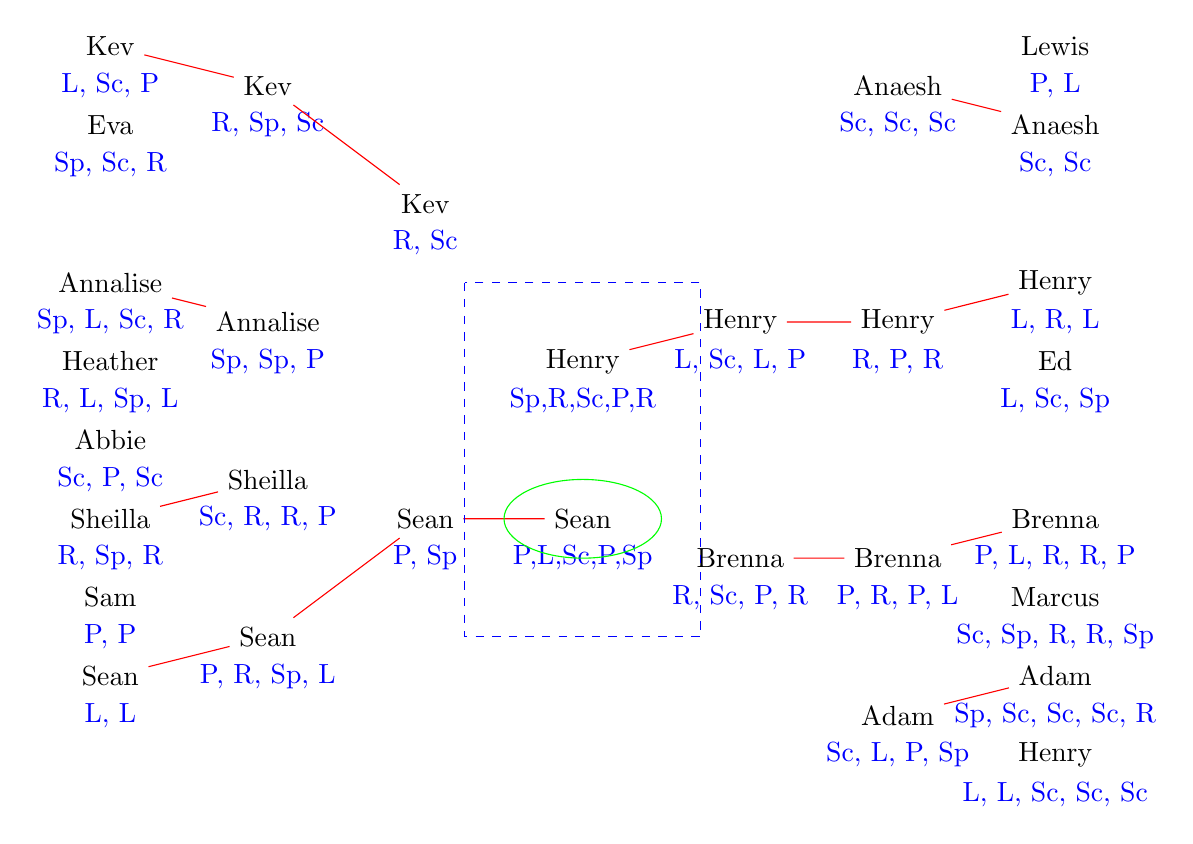
\begin{tikzpicture}
        % First round
        % Duel 1
        \node (Kev) at (0,0) {Kev};
        \node at ($(Kev) + (0,-.5)$) [blue] {L, Sc, P};

        \node (Eva) at ($(Kev) + (0,-1)$) {Eva};
        \node at ($(Eva) + (0,-.5)$) [blue] {Sp, Sc, R};

        % Duel 2
        \node (Annalise) at ($(Eva) + (0,-2)$) {Annalise};
        \node at ($(Annalise) + (0,-.5)$) [blue] {Sp, L, Sc, R};

        \node (Heather) at ($(Annalise) + (0,-1)$) {Heather};
        \node at ($(Heather) + (0,-.5)$) [blue] {R, L, Sp, L};

        % Duel 3
        \node (Abbie) at ($(Annalise)+(0,-2)$) {Abbie};
        \node at ($(Abbie) + (0,-.5)$) [blue] {Sc, P, Sc};

        \node (Sheilla) at ($(Abbie) + (0,-1)$) {Sheilla};
        \node at ($(Sheilla) + (0,-.5)$) [blue] {R, Sp, R};

        % Duel 4
        \node (Sam) at ($(Abbie) + (0,-2)$) {Sam};
        \node at ($(Sam) + (0,-.5)$) [blue] {P, P};

        \node (Sean) at ($(Sam) + (0,-1)$) {Sean};
        \node at ($(Sean) + (0,-.5)$) [blue] {L, L};

        % Duel 5
        \node (Lewis) at (12,0) {Lewis};
        \node at ($(Lewis) + (0,-.5)$) [blue] {P, L};

        \node (Anaesh) at ($(Lewis) + (0,-1)$) {Anaesh};
        \node at ($(Anaesh) + (0,-.5)$) [blue] {Sc, Sc};

        % Duel 6
        \node (Henry) at ($(Anaesh) + (0,-2)$) {Henry};
        \node at ($(Henry) + (0,-.5)$) [blue] {L, R, L};

        \node (Ed) at ($(Henry) + (0,-1)$) {Ed};
        \node at ($(Ed) + (0,-.5)$) [blue] {L, Sc, Sp};

        % Duel 7
        \node (Brenna) at ($(Ed)+(0,-2)$) {Brenna};
        \node at ($(Brenna) + (0,-.5)$) [blue] {P, L, R, R, P};

        \node (Marcus) at ($(Brenna) + (0,-1)$) {Marcus};
        \node at ($(Marcus) + (0,-.5)$) [blue] {Sc, Sp, R, R, Sp};

        % Duel 8
        \node (Adam) at ($(Brenna) + (0,-2)$) {Adam};
        \node at ($(Adam) + (0,-.5)$) [blue] {Sp, Sc, Sc, Sc, R};

        \node (Henry1) at ($(Adam) + (0,-1)$) {Henry};
        \node at ($(Henry1) + (0,-.5)$) [blue] {L, L, Sc, Sc, Sc};

        % Second round
        % Duel 1
        \node (Kev_1) at ($(Kev) + (2,-.5)$) {Kev};
        \node at ($(Kev_1) + (0,-.5)$) [blue] {R, Sp, Sc};

        \node (Annalise_1) at ($(Annalise) + (2,-.5)$) {Annalise};
        \node at ($(Annalise_1) + (0,-.5)$) [blue] {Sp, Sp, P};

        % Duel 2
        \node (Sheilla_1) at ($(Sheilla) + (2,.5)$) {Sheilla};
        \node at ($(Sheilla_1) + (0,-.5)$) [blue] {Sc, R, R, P};

        \node (Sean_1) at ($(Sean) + (2,.5)$) {Sean};
        \node at ($(Sean_1) + (0,-.5)$) [blue] {P, R, Sp, L};

        % Duel 3
        \node (Anaesh_1) at ($(Anaesh) + (-2,.5)$) {Anaesh};
        \node at ($(Anaesh_1) + (0,-.5)$) [blue] {Sc, Sc, Sc};

        \node (Henry_1) at ($(Henry) + (-2,-.5)$) {Henry};
        \node at ($(Henry_1) + (0,-.5)$) [blue] {R, P, R};

        % Duel 4
        \node (Brenna_1) at ($(Brenna) + (-2,-.5)$) {Brenna};
        \node at ($(Brenna_1) + (0,-.5)$) [blue] {P, R, P, L};

        \node (Adam_1) at ($(Adam) + (-2,-.5)$) {Adam};
        \node at ($(Adam_1) + (0,-.5)$) [blue] {Sc, L, P, Sp};

        % Third round
        % Duel 1
        \node (Kev_2) at ($(Kev_1) + (2,-1.5)$) {Kev};
        \node at ($(Kev_2) + (0,-.5)$) [blue] {R, Sc};

        \node (Sean_2) at ($(Sean_1) + (2,1.5)$) {Sean};
        \node at ($(Sean_2) + (0,-.5)$) [blue] {P, Sp};

        % Duel 4
        \node (Henry_2) at ($(Henry_1) + (-2,0)$) {Henry};
        \node at ($(Henry_2) + (0,-.5)$) [blue] {L, Sc, L, P};

        \node (Brenna_2) at ($(Brenna_1) + (-2,0)$) {Brenna};
        \node at ($(Brenna_2) + (0,-.5)$) [blue] {R, Sc, P, R};

        % Final

        \node (Sean_3) at ($(Sean_2) + (2,0)$) {Sean};
        \node at ($(Sean_3) + (0,-.5)$) [blue] {P,L,Sc,P,Sp};

        \node (Henry_3) at ($(Henry_2) + (-2,-.5)$) {Henry};
        \node at ($(Henry_3) + (0,-.5)$) [blue] {Sp,R,Sc,P,R};

        % Connectors

        \draw [red] (Annalise) -- (Annalise_1);
        \draw [red] (Sheilla) -- (Sheilla_1);
        \draw [red] (Anaesh) -- (Anaesh_1);
        \draw [red] (Adam) -- (Adam_1);

        \draw [red] (Kev) -- (Kev_1) -- (Kev_2);
        \draw [red] (Brenna) -- (Brenna_1) -- (Brenna_2);

        \draw [red] (Henry) -- (Henry_1) -- (Henry_2) -- (Henry_3);
        \draw [red] (Sean) -- (Sean_1) -- (Sean_2) -- (Sean_3);

        % Lines and stuff

        \draw [blue, dashed] (4.5,-3) rectangle (7.5,-7.5);

        % Winner

        \draw [green] ($(Sean_3)$) ellipse  (1 and .5);

    \end{tikzpicture}
\end{document}
